\documentclass[a4paper,10pt,twoside]{IEEEtran}

\usepackage{graphicx}
\usepackage{placeins}
\usepackage{hyperref}
\usepackage{pdfpages}
\usepackage{fullpage}
\usepackage[bf]{caption}
\usepackage[english]{babel}
\usepackage{verbatim}
\usepackage{cite}
\usepackage{wrapfig}
\usepackage[marginpar]{todo}
\usepackage{paralist}
\usepackage{booktabs}
\usepackage{subcaption}
\usepackage{mathtools}
\usepackage{fancyhdr}
\usepackage{algpseudocode}
\usepackage{algorithm}
\usepackage{tikz}
%\usepackage{gnuplot-lua-tikz}
\usetikzlibrary{calc,intersections}
\usepackage{amssymb}

\hypersetup{
    colorlinks,
    pdftitle={Report Localization Option 1 IN4254 Smart Phone Sensing},
    pdfauthor={in4254-dhoepelman-mprovokluit},
}

\setlength{\parindent}{0pt}
\setlength{\parskip}{2ex}

\usepackage[utf8]{inputenc}
\usepackage[T1]{fontenc}

\newcommand{\axis}[1]{$#1$\nobreakdash-axis}
\newcommand{\plane}[2]{$#1#2$\nobreakdash-plane}

\title{\huge{\textbf{Report Localization Option 1}\\IN4254 Smart Phone Sensing}}
\date{\today}
\author{David Hoepelman (1521969) \and Mark Provo Kluit (1263099)}

\setlength{\headheight}{15pt}
\addtolength{\headsep}{15pt} % no love between header and main text
%\addtolength{\textheight}{-20pt} % more space between text and empty footer

\pagestyle{fancy}
 
\fancyhf{}
\fancyhead[LE,RO]{thepage}
\fancyhead[RE]{\textit{\nouppercase{\leftmark}}}
\fancyhead[LO]{\textit{\nouppercase{\rightmark}}}
 
\fancypagestyle{plain}{ %
\fancyhf{} % remove everything
\renewcommand{\headrulewidth}{0pt} % remove lines as well
\renewcommand{\footrulewidth}{0pt}}

\begin{document}

\maketitle

\section{Data collection}
\label{sec:localization-method}

\begin{figure}
  \centering
    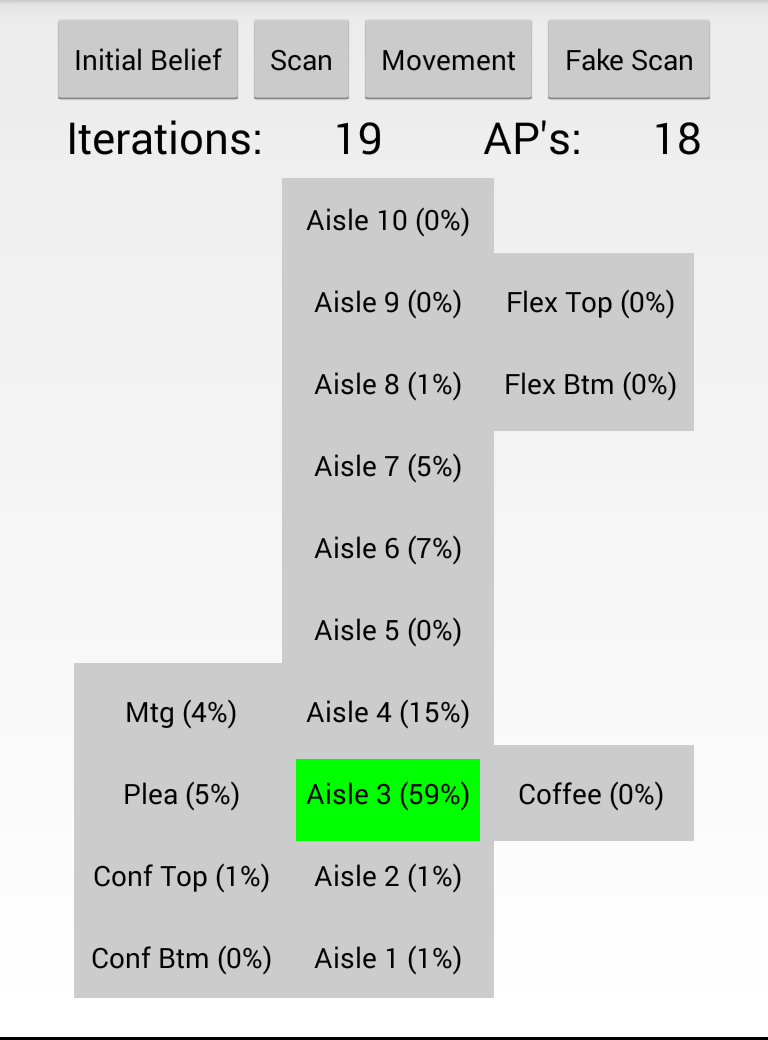
\includegraphics[width=0.36\textwidth]{screenshot}
    \label{fig:screenshot}
    \caption{GUI showing successful localization}
\end{figure}

We collected WiFi data for the mandated 17 cells, which we call rooms.
A rough not-to-scale map can be seen in our GUI (Figure \ref{fig:screenshot}).

In total we collected \textbf{3300} scans for WiFi access points on 3 different dates.
A scan lists all detectable \emph{access points} (APs) as a list of $signal=(BSSID, SSID, level)$ tuples where $level$ was expressed in dBm and was in $[-30,-100]$.
Both 2.4Ghz and 5Ghz access points were detected.
Most rooms have 180 or 240 scans, depending on which days they were accessible.
The collected scans inside a room were evenly divided among the room area.

On average each scan contained 20.0 $BSSID$'s, although the number varied per room.
We did a fixed number of scans per room on every day, but this does not translate well into a sampling time per cell.
The reason for this is that the time for a signal scan differed greatly depending on the number of APs visible.

\newpage

\section{Localization method}
\label{sec:data}

We chose to use \textbf{Bayesian Filters} for our localization method. We uniquely identify an AP using the $BSSID$, which is guaranteed globally unique.

For our calculations we group the the training data on $BSSID$ and $Room$ and calculate the normal distribution $N_{BSSID,Room}(\mu_{BSSID,Room}, \sigma^2_{BSSID,Room})$.

We ignore a signal if it had the $SSID$ (network name) "TUvisitor", "tudelft-dastud" or "Conferentie-TUD".
This is because most of the TU Delft access points sent out 4 different $SSID$'s (the other is "eduroam") with different $BSSID$'s.
As these signals come from the same physical location and have the same frequency (and probably the same radio hardware) we did not think they would add more information, and at worst might make our results more inaccurate (by processing essentially the same signal 4 times, thus biasing the results heavily on those AP's).

For localization we express the location as a probability vector $\mathbf{loc}$, with $\mathbf{loc}_{r}$ being the probability that we are in room $r$. 
We initially start with the \emph{intial belief}: where each location has even probability $\mathbf{loc}_r = \frac{1}{|\mathbf{loc}|}$.
We then do a WiFi scan which gives a list of signals.
We sort this list on level, with strongest level first.
As long as the largest probability is under a threshold $0.95$ we then iterate the list, while adjusting the location each iteration.
The location is adjusted by getting for each room the chance of that signal level and multiplying it with the existing probability. After each iteration we normalize $loc$ by making it sum to 1.
\\
\begin{algorithmic}
	\State $scan \gets \text{list of } (BSSID, SSID, level) \text{ sorted on }level$
	\While {$\max{\mathbf{loc}} < 0.95$}
		\State $signal \gets \text{next } scan$
		\ForAll{$Room$}
			\State $p \gets N_{BSSID,Room}(level-0.5,level+0.5)$
			\State $\mathbf{loc}_{Room} \gets \mathbf{loc}_{Room} \cdot p $
		\EndFor
		\State \text{normalize} $\mathbf{loc}$
	\EndWhile
\end{algorithmic}

We retain $\mathbf{loc}$ between scans, unless the locator is reset to its initial belief.

\subsection{Number of access points}
\label{subsec:numap}

While we achieved a pretty good accuracy with pure bayesian filters (see performance evaluation section) we later added another probability based on the number of access points that was visible.
For this we created the normal distribution $N_{\#,Room}$ from the training data, which gives the distribution of number of APs in a scan based on the $\mu$ and $\sigma$ of the number of APs per room in the training data.
This helped in rooms where not a lot of signals were measurable. Thus we appended to the previous algorithm:
\begin{algorithmic}
	\If {$\max{\mathbf{l}} < 0.95$}
		\ForAll{$Room$}
			\State $p \gets N_{\#,Room}(|scan|-0.5,|scan|+0.5)$
			\State $\mathbf{l}_{Room} \gets \mathbf{l}_{Room} \cdot p $
		\EndFor
		\State \text{normalize} $\mathbf{l}$
	\EndIf
\end{algorithmic}


\section{Performance evaluation}
\label{sec:evaluation}

For our performance evaluation we used off-line processing. We divided the scans of our training data into 10 random partitions, and tested every partition while using the other partitions as training data for the locator.

Using this method we achieved an accuracy of \textbf{83\%} (2731 of 3300).
While analyzing the data we saw that a lot of mis-classified scans were done in the \emph{Coffee} room.
We determined that this was because the scans in that room usually contained only 0-3 signals.
This is not enough for the bayesian filter.

To alleviate this problem we altered our code to take the number of visible signals into account.
This improved our accuracy to \textbf{89\%} (2945 of 3300).
The technical implementation for this is specified in section \ref{subsec:numap}.
If we mark adjacent rooms as correct too, which is not unreasonable as some training scans were taken on the border between rooms, our accuracy improves to \textbf{95\%} (3132 of 3300).

\newpage

\section{Discussion}
\label{sec:discussion}
TODO

Bayesian filters are not useful if you have cells where a low number of access points is visible.
Our trick to take the number of APs into accounts work well when the number of cells without much APs visible is low.
However if there are more cells like these, this approach will likely fail.
Another possibility we contemplated was to create a bitstring of present/not-present $BSSID's$ for the current scan and all training data.
By then computing the hamming distance to the training data points we can get more information which we can add to the probability filter.
This will more likely work in the general case.



\newpage

\addcontentsline{toc}{chapter}{Bibliography}
% styles: abbrv, ieeetr, plain
\bibliographystyle{abbrv}
\bibliography{report}

\newpage
\appendix



\end{document}
